

\documentclass[]{article}
\usepackage{amsmath}
\usepackage{amsthm}
\usepackage{amssymb}
\usepackage{graphicx}
\usepackage[utf8]{inputenc} 
\usepackage{subcaption}
\usepackage{caption}
\usepackage{hyperref}
\usepackage{amsbsy}
\usepackage[left=4cm]{geometry}
 %http://tex.stackexchange.com/questions/595/how-can-i-get-bold-math-symbols
%opening
\title{Variance reduction in coarse bifurcation analysis of stochastic models}
\author{Pieter Van Nuffel}

\newcommand{\R}{\ensuremath{\mathbb{R}}} % commando zonder argumenten
\newcommand{\C}{\ensuremath{\mathbb{C}}}
\newcommand{\N}{\ensuremath{\mathbb{N}}}
\newcommand{\E}{\ensuremath{\mathbb{E}}}
\newcommand{\norm}[1]{\left\|#1\right\|} % commando's met argumenten
\newcommand{\pa}[2]{\frac{\partial #1}{\partial #2}}
\newcommand{\ppa}[2]{\frac{\partial^2 #1}{\partial #2^2}}
\newcommand{\dd}{\ensuremath{\mathrm{d}}}
\newcommand{\U}{\ensuremath{\boldsymbol{\rho}}}
\newcommand{\cts}{\ensuremath{\boldsymbol{\Phi}^N_T}} %Coarse time step
\newcommand{\V}{\ensuremath{\mathbf{v}}} 
\newcommand{\jv}{\ensuremath{\mathbf{\hat{Jv}}}}
\newcommand{\jvpde}{\ensuremath{\mathbf{Jv}_{FP}}}

\theoremstyle{definition}
\newtheorem{Theorem}{Theorem}


\begin{document}
\subsubsection{Nota's}
Tijdens elke continueringsstap, wordt een nieuw punt gecreëerd dat initieel de dichtheid \U krijgt van het vorig punt en met een parameter (D) die horizontaal word geupdate. Dan wordt de norm van het residu berekend $\norm{ \U(t) - \U(t+\Delta t)} $, waarin de dichtheid op de volgende tijdsstap verkregen wordt door een simulatie van het systeem met de nieuwe parameter. De grootte van het residu is dus afhankelijk van de stapgrootte in de bifurcatieparamter. De newtontolerantie is de norm van het residu. Als de newton-tolerantie te groot gekozen wordt (in vergelijking met de stapgrootte van het residu), dan wordt er geen Newton-iteratie uitgevoerd. Als de Newton-tolerantie evenwel te klein gekozen wordt, dan bereikt de Newton-solver mogelijk geen convergentie ten gevolge van de ruis. De Newton-tolerantie moet dus weloverwogen gekozen worden. 



\subsection{Results for the pde}
Ook hier zien we dat de keuze van de newtontolerantie belangrijk is (te groot = kans op dezelfde toestanden , te klein= failed iterations).
Dit kan echter opgevangen worden door de oplossing van dx nauwkeuriger te maken door de tolerantie van de GMRES te verfijnen (het probleem was dat er dx=0 oplossingen werden teruggegeven) 

\begin{figure}
%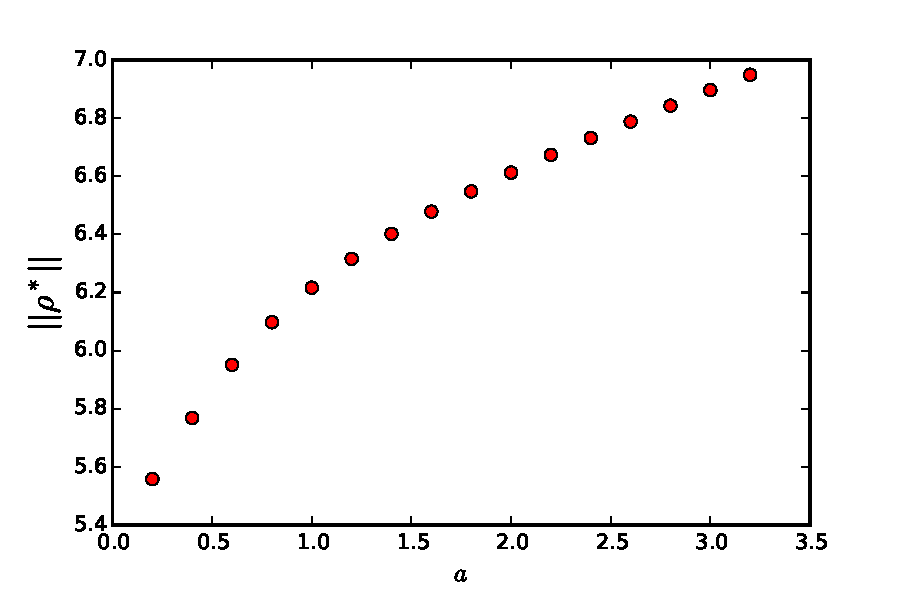
\includegraphics{../Problems/WeightedParticles/checkSystem/plots/bifurcation_pde(D)}
\caption{  Bifurcation diagram of the steady states calculated with the Newton-Krylov-Solver for the PDE. $\Delta t = 10^{-4}, \Delta T = 10^{-2}, \Delta x = 10^{-2}, \Delta D = 0.01, \epsilon_{GMRES}=10^{-5},  \delta_{Newton} = 10^{-7}, \epsilon=10^{-5}$
}
\end{figure}

\subsection{Results for the sde}
We chose $\Delta \sigma = 0.05$ as continuation step seize. Performing a bifurcation with smaller steps is pointless, because the difference in densities will become too small in comparison with the noise on the residual.

\begin{figure}
%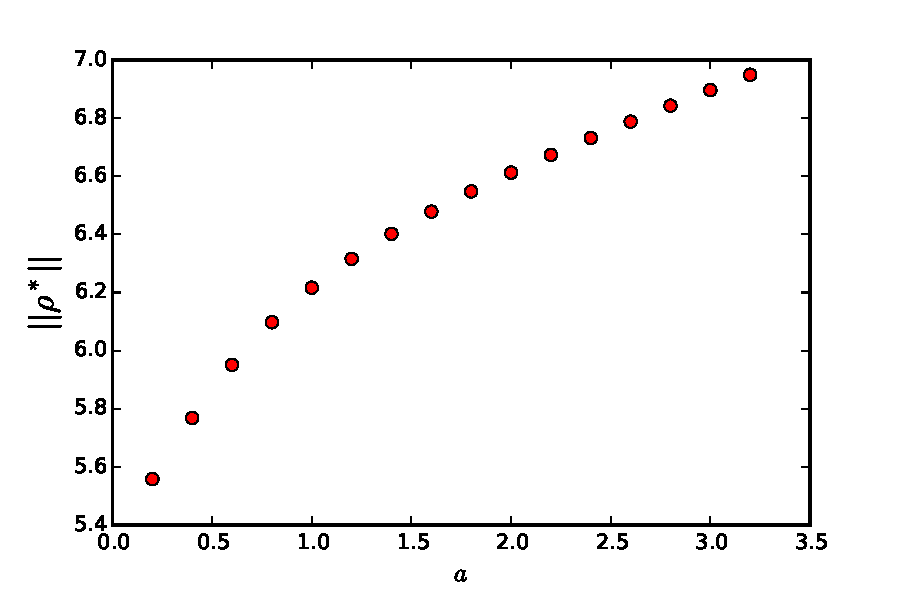
\includegraphics{../Problems/WeightedParticles/checkSystem/plots/bifurcation_pde(D)}
\caption{  Bifurcation diagram of the steady states calculated with the Newton-Krylov-Solver for the SDE. $\Delta t = 10^{-3}, \Delta T = 10^{-1}, \Delta x = 10^{-2}, \epsilon_{GMRES}=10^{-5},  \delta_{Newton} = 10^{-7}, \epsilon=10^{-5}$
}
\end{figure}

%\begin{center}
%\begin{table}
%\caption{Parameter values}
%  \begin{tabular} { | c  | c |}    \hline   
%     %FTCS-scheme  &   Euler-Maruyama-scheme  \\  
%   \textit{ {Discretization parameters}}&    &  SDE    \\ \hline
%       $\Delta t $  & $10^{-4}$ \\ 
%       $\Delta T $ &  $10^{-2}$ \\ 
%      $ \Delta x &  $10^{-2}$ \\ 
%       $ \Delta D$  $  &  $ 0.01 $ \\ \hline
%  \end{tabular}
%\end{table}
%\end{center}

\end{document}